\documentclass[12pt, a4paper, oneside]{book}   	% document style definition


\usepackage{hslu}                               % apply HSLU style
\usepackage{comment}                            % having comment sections \begin{comment} \end{comment}
\usepackage[utf8]{inputenc}						% charactere interpretation
\usepackage{amsmath}							% math package
\usepackage{amsfonts}							% font package for math symbols
\usepackage{amssymb}							% symbols package - definition of math symbols
\usepackage{listings}							% package for code representation

\usepackage{csquotes}       % Quotation support
\usepackage[style=apa,backend=biber]{biblatex}       % Bibliography, 
% todo: original template uses ieee3
\addbibresource{references.bib} % Bibliography file

\usepackage{graphicx}							% for inclusion of image
\setlength {\marginparwidth }{2cm}
\usepackage{todonotes}
\renewcommand{\todo}[1]{\textcolor{red}{TODO: #1}}
%\presetkeys{todonotes}{inline, textcolor=red, color=none, noinlinepar}{}

%\let\todoold\todo
%\newcommand{\todo}[1]{\textcolor{red}{TODO: #1}\todo[prepend, caption={TODO: #1}]{}}

%\renewcommand{\todo}[1]{\todo[inline]{\textcolor{red}{TODO: #1}}}
%\renewcommand{\todo}[1]{\todo{\textcolor{red}{TODO: #1}}}




\usepackage{booktabs}       % Better tables
\usepackage{caption}        % Better captions
\usepackage{subfig}								% to arrange figures next to each other
\usepackage{float}								% text style surrounding images
\usepackage{threeparttable}
\usepackage{tikz}								% used to place logos on title page
% \usepackage{gensymb}							% for special characters such as °
\usepackage{titlesec}
\usepackage{multirow}
\usepackage{siunitx}
\usepackage{tabularx}
\usepackage{tikzscale}


% PDF/A Compliance, todo: enable and remove hyperref usepackage afterwards
% \usepackage[a-1b]{pdfx}
% \catcode30=12

\usepackage{hyperref}
\hypersetup{hidelinks}

\usepackage[acronym]{glossaries}         				% package for glossary

\setcounter{tocdepth}{1}                        % hide subsections from TOC
\makenoidxglossaries
\newacronym{HSLU}{HSLU}{Lucerne University of Applied Sciences and Arts}
\newacronym[see={[Glossary:]{fitzpatrick-skin-type}}]{FST}{FST}{Fitzpatrick skin type\glsadd{fitzpatrick-skin-type}}
\newacronym{ML}{ML}{Machine Learning}
\newacronym{AI}{AI}{Artificial Intelligence}
\newacronym{FPR}{FPR}{false positive rate}
\newacronym{TPR}{TPR}{true positive rate}
                                % include acronyms.txt file
\newglossaryentry{fitzpatrick-skin-type}{
	name={Fitzpatrick skin type},
	plural={Fitzpatrick skin types},
	description={A skin classifier based on the skins' reaction to ultraviolet light, developed by dermatologist Dr. Thomas Fitzpatrick \autocite{Gottfrois2024}}
}
\newglossaryentry{JupyterNotebook}{
	name={Jupyter Notebook},
	description={Executable files, often used in ML to write Python code and add explanations in text form}
}
\newglossaryentry{gpuhub}{
	name={GPUhub},
	description={\gls{HSLU}’s server infrastructure for GPU-related computing. It provides isolated environments with JupyterLab access for developing and running \gls{ML} workflows}
}
\newglossaryentry{pediatric}{
	name={pediatric},
	description={A medical term for infants, children and adolescents \autocite{Farlex_nodate}}
}
\newglossaryentry{proxyVar}{
	name={proxy variable},
	plural={proxy variables},
	description={"one or more variables that encode the protected attribute with a substantial degree of accuracy" \autocite{Wang_2021}}
}
\newglossaryentry{teledermatology}{
	name={teledermatology},
	description={dermatological care from a distance, supported by modern technology \autocite{Pala_2020}}
}
\newglossaryentry{Fairlearn}{
	name=Fairlearn,
	description={A Python library for assessing and improving fairness in machine learning models. It supports various fairness metrics and mitigation techniques, especially for binary classification tasks \autocite{Fairlearn_nodate}}
}
\newglossaryentry{Equalized-Odds-Difference}{
	name={equalized odds difference},
	description={The absolute difference in true positive and false positive rates between subgroups, used as a group fairness metric \autocite{Fairlearn_nodate}}
}
\newglossaryentry{Equalized-Odds-Ratio}{
	name={equalized odds ratio},
	description={The ratio of true positive and false positive rates between subgroups, used as a group fairness metric \autocite{Fairlearn_nodate}}
}                                % include glossary.txt file
\graphicspath{{figures/}}						    % set path of graphics folder




% Format chapter titles without "Chapter X" prefix
\titleformat{\chapter}[hang]
{\normalfont\LARGE\bfseries}  % Style: Large bold text
{\thechapter}                 % Number format: Just the number
{1em}                         % Space between number and title
{}                            % Code before the title (empty)



%----------------------------------------------------------------------------------------
%	DOCUMENT INFORMATION
%----------------------------------------------------------------------------------------
\author{Nadja Stadelmann}                       % author name
\city{Lucerne (Switzerland)}                    % author's place of origin
\title{Demographic Biases in\linebreak Dermatology Models}   % thesis title
\subtitle{\large \todo{subtitle}}               % thesis subtitle

\date{2025}                                     % the year when the thesis was written (for the titlepage)
\defensedate{\todo{adapt date} October 27th, 2024}                % the date of the private defense
\defencelocation{Lucerne}                       % location of defence
\extexpert{Dr. Jürg Schelldorfer}                         % name of external expert
\indpartner{Applied AI Research Lab}                       % name of industry partner

% jury, supervisor and dean are only relevant if acceptance sheet is enabled with the next line
% \acceptsheet
\jury{                                          % members of the jury
    \begin{itemize}
        \item Prof. Dr. Name Surname from Lucerne University of Applied Sciences and Arts, Switzerland (President of the Jury);
        \item Prof. Dr. Name Surname from Lucerne University of Applied Sciences and Arts, Switzerland (Thesis Supervisor);
        \item Prof. Dr. Name Surname from Lucerne University of Applied Sciences and Arts, Switzerland (External Expert).
    \end{itemize}
}

\supervisor{Dr. Ludovic Amruthalingam}             % name of supervisor
\dean{Prof. Dr. René Hüsler}                   % name of faculty dean

\acknowledgments{Thanks to my family, relatives and friends for all the support given to finish this thesis.
	\todo{add thanks and gratitude}
	Ludovic Amruthalingam
	Simone Lionetti - deputy Ludovic
	Pascal Baumann - LaTeX
	Philippe Gottfrois - information and work on PASSION project
}


\begin{document}
	\english                                        % define thesis language: \german or \german
	\maketitle
	
	
	%----------------------------------------------------------------------------------------
	%	PREAMBLE
	%----------------------------------------------------------------------------------------
	\begin{abstractstyle}{\hsummary}
		\todo{Your abstract here.}
	    The content of your thesis in brief.
	\end{abstractstyle}
	
	\tableofcontents
	
	\listoftodos
	\todo{solve todos} 
	
	
	\todo{also solve todos in the code ;)} 
	
	
	\todo{also fix metadata entry!!!} 
	
	
	\todo{Alle Fakten (fundiertes Wissen Dritter) sind korrekt zitiert. Es werden verschiedene Zitierweisen verwendet und teilweise mehrere Interpretationen gegenübergestellt. Der gemeinsam definierte Zitierstil im Text, in Abbildungen und Tabellen sowie im Literaturverzeichnis wird korrekt und durchgängig angewendet. Eigene Leistungen (sowie Bewertungen) und Fremdquellen sowie Recherchen sind klar unterscheidbar.} 
	
	
	\todo{Die erstellten Artefakte sind von sehr hoher Qualität. Das trifft u.a. auf Diagramme, Skizzen sowie Notationen (z.B. BPMN/UML) zu. Darstellungen sind einwandfrei, alle statistisch notwendigen Qualitätskriterien sind erfüllt. Beschriftungen etc. sind vorhanden, keine Einwände, Text und Bild stimmen beschreibend gut überein. Es wurden angemessene Dokumentationsmethoden und -arten korrekt verwendet. Vereinbarte Interview Transkripte, Beobachtungsprotokolle bzw. Zusammen-fassungen sind vorhanden. Daten, Ort, Kontext, Beschreibung, Zeilennummer, Verweise, Strukturen sind erkennbar, gut formatiert und korrekt mit dem Text/ der Analyse verknüpft. Alle Elemente und Themen sind im methodischen Teil/Text erklärt und verständlich, keine technischen oder strukturellen Einwände. Auch Zwischenanalysen, Zwischenschritte oder Gesamtauswertungen wurden durchgeführt, die Herkunft der Daten ist erkennbar und professionell aufbereitet.} 
	
	
	\todo{Der Schreibstil aller Dokumente entspricht hohen Standards und enthält keine Übertreibungen oder unbegründete Beurteilungen. Die Sprache ist aussagekräftig, prägnant und präzise. Die Fachterminologie ist konsistent, d.h. für gleiche Gegenstände und Themen werden immer die gleichen Begriffe verwendet. Der Sprachgebrauch ist durchgängig geschlechtergerecht, einheitlich und sachlich.}


	\todo{Portfolio DB für Referenzarbeiten anschauen}
	
	\listoffigures
	\listoftables
	% print list of acronyms and glossary
	\printnoidxglossaries
	
	
	
	%----------------------------------------------------------------------------------------
	%	MAIN CONTENT
	%----------------------------------------------------------------------------------------
	\mainmatter
	
	% write or compose the main document here
	
	\chapter{Problem Statement}
		\todo{Welche Ziele, Fragestellungen werden mit dem Projekt verfolgt? Die Bedeutung, Auswirkung und Relevanz dieses Projektes für die unterschiedlichen Beteiligten soll aufgeführt werden. Typischerweise wird hier ein Verweis auf die Aufgabenstellung im Anhang gemacht.}
	
		\todo{Formulate statement from those citations}:
		\begin{itemize}
			\item AI systems can be used in many sensitive environments to make important and life-changing decisions; thus, it is crucial to ensure that these decisions do not reflect discriminatory behavior toward certain groups or populations \autocite{Mehrabi_2021}.
			\item There are clear benefits to algorithmic decision-making; unlike people, machines do not become tired or bored [45, 119], and can take into account orders of magnitude more factors than people can. However, like people, algorithms are vulnerable to biases that render their decisions “unfair” [6, 121]. In the context of decision-making, fairness is \textit{the absence of any prejudice or favoritism toward an individual or group based on their inherent or acquired characteristics}. Thus, an unfair algorithm is one whose decisions are skewed toward a particular group of people. \autocite{Mehrabi_2021}.
			\item it is important for researchers and engineers to be concerned about the downstream applications and their potential harmful effects when modeling an algorithm or a system \autocite{Mehrabi_2021}.
			\item We should think responsibly, and recognize that the application of these tools, and their subsequent decisions affect peoples’ lives; therefore, considering fairness constraints is a crucial task while designing and engineering these types of sensitive tools \autocite{Mehrabi_2021}.
		\end{itemize}
	
	
		\section{Context}
			This thesis is part of the PASSION project. The PASSION research team identified that in Africa, dermatology treatment is not accessible. There is less than one dermatologist per one million citizens. In contrast, there is high demand for dermatology treatment, especially among children and adolescents. 80\% of the \gls{pediatric} population is affected. The goal of PASSION is to make dermatology treatment more accessible by using AI supported telemedicine for triage \autocite{Gottfrois2024}.
			
			For AI supported triage, demographic biases in existing dermatology models is a problem since the corresponding datasets lack diversity, especially regarding skin tones \autocite{Gottfrois2024}. This type of bias is important in dermatology, since different diseases present themselves differently depending on the skin-color \autocite{Diaz2022}. Further, skin diseases are more advanced or severe at diagnosis in patients with lower socioeconomic status \autocite{BAD2021}.
			
			PASSION tries to mitigate the demographic bias by providing a dataset of pigmented skin images of patients from Sub-Saharan Africa. The PASSION team focused on gathering data with \gls{FST} IV, V and VI. Further, the covered conditions represent up to 80\% of the conditions in the \gls{pediatric} population, the demographic group who is most affected by skin disease \autocite{Gottfrois2024}. \gls{HSLU}
			
			The PASSION dataset is complementary to the existing datasets and improves the diversity in a combined dataset. Within the dataset itself, there could potentially be further demographic biases, e.g. related to age or gender.
	
		\section{Objective}
			The goal of this research is to
			\begin{enumerate}
				\item Identify demographic biases in dermatology AI models, using established fairness metrics.
				\item Identify mitigation strategies to minimize these biases.
				\item Assess the effectiveness of the mitigation strategies.
			\end{enumerate}
			It is important to identify the existent biases first, so that the mitigation strategies can be \todo{proceed here to reason why you chose those objectives}
	
	\chapter{State of Research}
		\todo{Bezogen auf die eigenen Zielsetzungen und Fragestellungen soll aufgezeigt werden, wie andere dieses oder ähnliche Probleme gelöst haben. Worauf können Sie aufbauen, was müssen Sie neu angehen?	Wodurch unterscheidet sich Ihre Lösung von anderen Lösungen? Für wissenschaftlich orientierte Arbeiten sei hier explizit auf (Balzert, S. 66 ff) verwiesen.}
		\todo{Relevante, aktuelle und fundierte Fachliteratur wurde identifiziert, kritisch geprüft und verwendet. Die Begriffe der Fragestellung sind definiert und referenziert. Der gesamte Kontext ist verknüpft und eine Abgrenzung wurde vorgenommen. All dies ist in einer leicht verständlichen Struktur formuliert und überprüft.}
		
		
		\section{PASSION for Dermatology}
			The PASSION research team provides a dataset including three analysis scripts and an AI model. For this thesis, it is important to understand which labels the dataset provides, so that the applicable bias mitigation methodologies can be chosen.
			
			The provided analysis scripts show a first insight into the demographic distribution in the dataset, such as Fitzpatrick skin type and cases per country distribution. The results of those analyses reveal first biases.
			
			There are also dermatology specific analysis scripts in regards of body localization by condition or impetigo cases. Those results 
			
			\subsection{PASSION Dataset}
				The PASSION dataset contains data from patients from four African countries. It contains 4901 images of dermatology cases and the corresponding demographic and clinical information, see \autoref{tab:PASSION_labels}. There is one record per patient and one or more corresponding images. The images are linked with the record by filename, which contains the subject\_id of the row entry. Access to the dataset can be requested via \href{https://passionderm.github.io/}{https://passionderm.github.io/} \autocite{Gottfrois2024}.
				
				\begin{table}[H]
					\centering
					\begin{tabularx}{\textwidth}{>{\hsize=.27\hsize}X>{\hsize=.27\hsize\raggedright}X>{\hsize=.46\hsize}X}
						\toprule
						\textbf{Label}       & \textbf{Data Type} & \textbf{Description}       \\ \midrule
						subject\_id          & string & Participant's unique identifier        \\
						country              & string & Country of origin of the participant   \\
						age                  & integer & Age of the participant in years       \\
						sex                  & m/f/o & Gender of the participant               \\
						fitzpatrick          & integer & \gls{FST}                \\
						body\_loc            & string (list; null-able, semicolon-separated) & Specific affected body locations \\
						impetig              & 0/1  & Presence of impetigo (1=present), may occur alone or with other conditions, affects the treatment options for coexisting conditions        \\
						conditions\_PASSION  & Eczema, Scabies, Fungal, Others & Primary diagnosed skin condition \\
						\bottomrule
					\end{tabularx}
					\caption{PASSION dataset - labels and descriptions \autocite{Gottfrois2024}}
					\label{tab:PASSION_labels}
				\end{table}
			
			\subsection{PASSION Analysis Scripts}
				With the Dataset, the PASSION research team provides a \gls{JupyterNotebook} with code examples and analysis scripts. They are listed in \autoref{tab:PASSION_scripts} with a description and an indicator, how relevant the scripts are for this thesis.
				\begin{table}[H]
					\centering
					\begin{tabularx}{\textwidth}{>{\hsize=.25\hsize\raggedright}X>{\hsize=.41\hsize}X>{\hsize=.34\hsize}X}
						\toprule
						\textbf{Script Title}       & \textbf{Description} & \textbf{Relevance - Reasoning}       \\ \midrule
						Linking CSV Data with Image Files & 
						Creates mapping between the data records and images. It further counts the cases by country  &
						\textbf{High} - Basis for other analysis's, potentially provides dermatological info        \\
						\hline
						Extracting and Comparing Subject IDs &
						Checks the dataset complecity and accurracy in regards of linking records and images &
						\textbf{Low} - Checks loaded data for completeness, but is not providing more insight   \\
						\hline
						Regrouping Malawi and Tanzania to EAS &
						data aggregation due to dataset size and geographical proximity &
						\textbf{Low} - Might be relevant to understand the dataset and for interpreting the results of the following scripts correctly  \\
						\hline
						Conditions by Country &
						Relationship between clinical conditions and country &
						\textbf{Medium} - Currently unsure whether this information is relevant for this thesis \todo{research relevance between country vs. clinical conditions in regards of demographic bias} \\
						\hline
						Body Localizations by Conditions &
						Shows correlation between the condition and primarily affected body parts; does not use all affected body parts listed in the data \todo{check with Philippe why this was done} &
						\textbf{Low} - While the correlation can be interesting for other research, it is not relevant for demographic biases. \\
						\hline
						Impetigo Cases            &
						Counts total number of impetigo cases as well as proportion to all cases &
						\textbf{Medium} - Currently unsure whether this information is relevant for this thesis \todo{research relevance between impedigo and demographic bias} \\
						\hline
						Distribution of Fitzpatrick Skin Types &
						Counts and visualizes the skin type distribution  &
						\textbf{High} - \gls{FST} is a demographic information   \\
						\bottomrule
					\end{tabularx}
					\caption{PASSION dataset - existing analysis scripts \autocite{Gottfrois2024} \todo{decide on a table style}}
					\label{tab:PASSION_scripts}
				\end{table}	
				
			\subsection{PASSION Experiments}
				see https://github.com/Digital-Dermatology/PASSION-Evaluation
			
			
		\section{General ML biases}
		
			\subsection{Discrimination vs. Biases}
			\begin{itemize}
				\item bias and discrimination = source of unfairness. Discrimination can be considered as a source for unfairness that is due to human prejudice and stereotyping based on the sensitive attributes, which may happen intentionally or unintentionally, while bias can be considered as a source for unfairness that is due to the data collection, sampling, and measurement. Although bias can also be seen as a source of unfairness that is due to human prejudice and stereotyping, in the algorithmic fairness literature it is more intuitive to categorize them as such according to the existing research in these areas. In this survey, we mainly focus on concepts that are relevant to algorithmic fairness issues. \autocite{Mehrabi_2021}
				\item Explainable Discrimination. Differences in treatment and outcomes amongst different groups can be justified and explained via some attributes in some cases. In situations where these differences are justified and explained, it is not considered to be illegal discrimination and hence called explainable [77]. In [77], authors present a methodology to quantify the explainable and illegal discrimination in data. They argue that methods that do not take the explainable part of the discrimination into account may result in non-desirable outcomes, so they introduce a reverse discrimination which is equally harmful and undesirable. They explain how to quantify and measure discrimination in data or a classifier’s decisions which directly considers illegal and explainable discrimination.\autocite{Mehrabi_2021}
				\item Unexplainable Discrimination. In contrast to explainable discrimination, there is unexplainable discrimination in which the discrimination toward a group is unjustified and therefore considered illegal. Authors in [77] also present local techniques for removing only the illegal or unexplainable discrimination, allowing only for explainable differences in decisions. These are preprocessing techniques that change the training data such that it contains no unexplainable discrimination. We expect classifiers trained on this preprocessed data to not capture illegal or unexplainable discrimination. Unexplainable discrimination consists of direct and indirect discrimination.\autocite{Mehrabi_2021}
				\begin{itemize}
					\item Direct Discrimination. Direct discrimination happens when protected attributes of individuals explicitly result in non-favorable outcomes toward them [164]. ... these traits that are considered to be “protected” or “sensitive” attributes in computer science literature  \autocite{Mehrabi_2021}
					\item Indirect Discrimination. In indirect discrimination, individuals appear to be treated based on seemingly neutral and non-protected attributes; however, protected groups, or individuals still get to be treated unjustly as a result of implicit effects from their protected attributes \autocite{Mehrabi_2021}
				\end{itemize}
				\item Discrimination can be either direct or indirect. Direct discrimination occurs when decisions are made based on sensitive attributes. Indirect discrimination occurs when decisions are made based on nonsensitive attributes which are strongly correlated with biased sensitive ones \autocite{M62_}
			\end{itemize}
			
			\subsection{Bias Introduction}
			\begin{itemize}
				\item These biased predictions stem from the hidden or neglected biases in data or algorithms \autocite{Mehrabi_2021}.
				\item two potential sources of unfairness in machine learning outcomes - those that arise from biases in the data and those that arise from the algorithms ... we observe that biased algorithmic outcomes might impact user experience, thus generating a feedback loop between data, algorithms and users that can perpetuate and even amplify existing sources of bias \autocite{Mehrabi_2021}.
				\item Bias in facial recognition systems [128] and recommender systems [140] have also been largely studied and evaluated and in many cases shown to be discriminative towards certain populations and subgroups. In order to be able to address the bias issue in these applications, it is important for us to know where these biases are coming from and what we can do to prevent them.\autocite{Mehrabi_2021}.
				\item We should think responsibly, and recognize that the application of these tools, and their subsequent decisions affect peoples’ lives; therefore, considering fairness constraints is a crucial task while designing and engineering these types of sensitive tools \autocite{Mehrabi_2021}.
				\item compared SAVRY, a tool used in risk assessment frameworks that includes human intervention in its process, with automatic machine learning methods in order to see which one is more accurate and more fair. Conducting these types of studies should be done more frequently, but prior to releasing the tools in order to avoid doing harm \autocite{Mehrabi_2021}.
				\item \textbf{Assessment Tools} An interesting direction that researchers have taken is introducing tools that can assess the amount of fairness in a tool or system. For example, Aequitas [136] is a toolkit that lets users to test models with regards to several bias and fairness metrics for different population subgroups. Aequitas produces reports from the obtained data that helps data scientists, machine learning researchers, and policymakers to make conscious decisions and avoid harm and damage toward certain populations. AI Fairness 360 (AIF360) is another toolkit developed by IBM in order to help moving fairness research algorithms into an industrial setting and to create a benchmark for fairness algorithms to get evaluated and an environment for fairness researchers to share their ideas [11]. These types of toolkits can be helpful for learners, researchers, and people working in the industry to move towards developing fair machine learning application away from discriminatory behavior \autocite{Mehrabi_2021}.
				\item At first sight, automating decisions may give a sense of fairness: classification rules do not guide themselves by personal preferences. However, at a closer look, one realizes that classification rules are actually learned by the system (e.g., loan granting) from the training data. If the training data are inherently biased for or against a particular community (e.g., foreigners), the learned model may show a discriminatory prejudiced behavior. In other words, the system may infer that just being foreign is a legitimate reason for loan denial. \autocite{M62_}
				\item One might think of a straightforward preprocessing approach consisting of just removing the discriminatory attributes from the data set. Although this would solve the direct discrimination problem, it would cause much information loss and in general it would not solve indirect discrimination. \autocite{M62_}
				\item Hence, there are two important challenges regarding discrimination prevention: one challenge is to consider both direct and indirect discrimination instead of only direct discrimination; the other challenge is to find a good tradeoff between discrimination removal and the quality of the resulting training data sets and data mining models. \autocite{M62_}
			\end{itemize}	
			
			\begin{itemize}
				\item Most AI systems and algorithms are data driven and require data upon which to be trained. Thus, data is tightly coupled to the functionality of these algorithms and systems. In the cases where the underlying training data contains biases, the algorithms trained on them will learn these biases and reflect them into their predictions. As a result, existing biases in data can affect the algorithms using the data, producing biased outcomes. Algorithms can even amplify and perpetuate existing biases in the data.\autocite{Mehrabi_2021}.
				\item In addition, algorithms themselves can display biased behavior due to certain design choices, even if the data itself is not biased. The outcomes of these biased algorithms can then be fed into real-world systems and affect users’ decisions, which will result in more biased data for training future algorithms.\autocite{Mehrabi_2021}.
				\item The loop capturing this feedback between biases in data, algorithms, and user interaction is illustrated in Figure 1. We use this loop to categorize definitions of bias in the section below \autocite{Mehrabi_2021}.
				\begin{figure}[H]
					\centering
					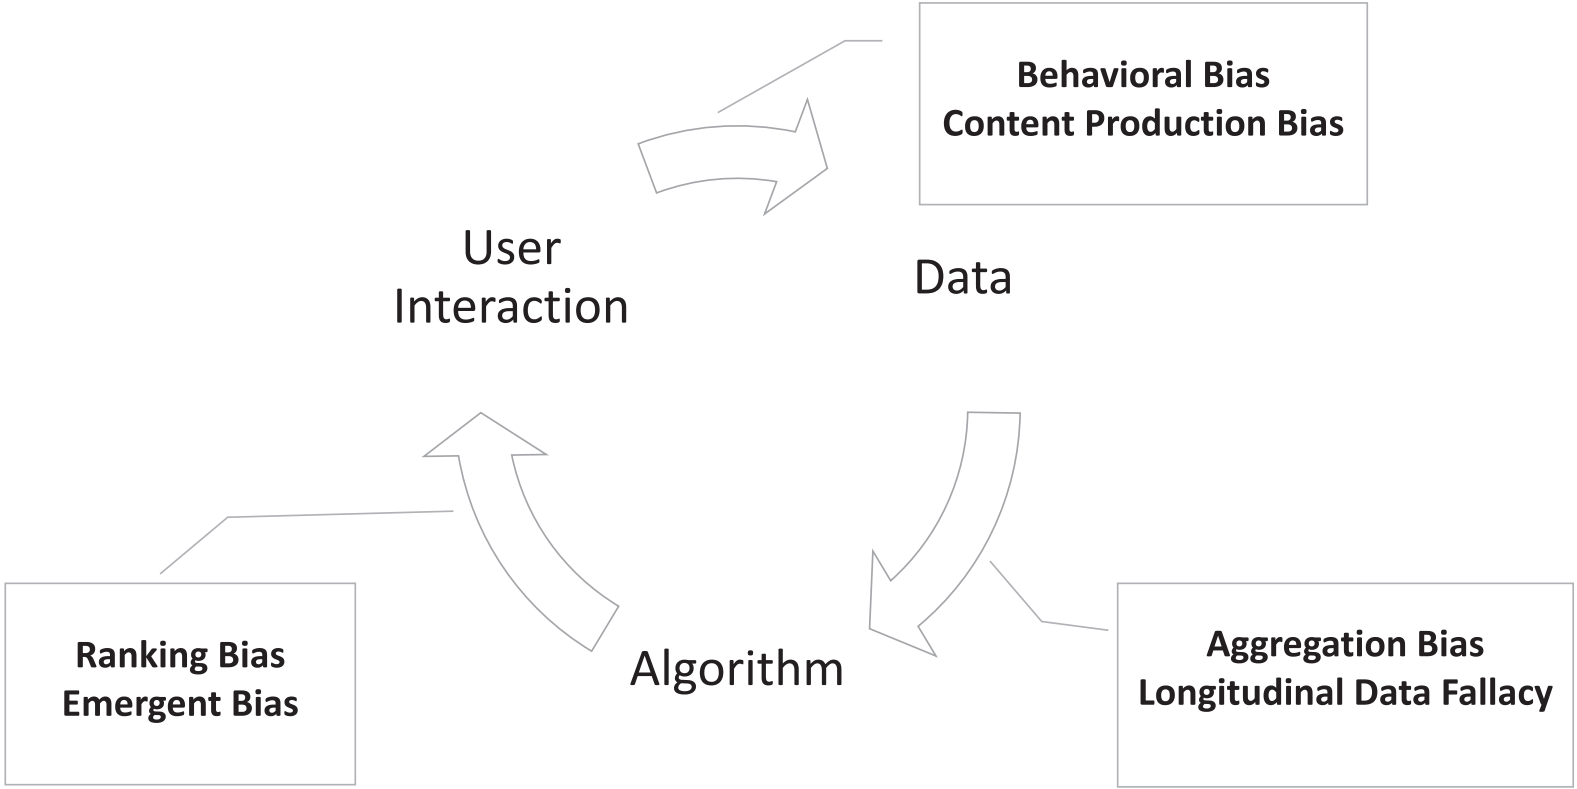
\includegraphics[width=0.8\textwidth]{figures/BiasCategoriesInMLLifecycle.png}
					\caption{Bias definitions in a ML lifecycle \autocite{Mehrabi_2021}.}
					\label{fig:example}
				\end{figure}
				\item Bias can exist in many shapes and forms, some of which can lead to unfairness in different downstream learning tasks. In \autocite{M144_Suresh_2021}, authors talk about sources of bias in machine learning with their categorizations and descriptions in order to motivate future solutions to each of the sources of bias introduced in the paper. In \autocite{M120_Olteanu_2019}, the authors prepare a complete list of different types of biases with their corresponding definitions that exist in different cycles from data origins to its collection and its processing.\autocite{Mehrabi_2021}.
			\end{itemize}	
			
			Already rewritten: The following categorization was modeled with the intent to show that the different biases are intertwined and one should consider the effects between each other in the cycle to address them correctly \autocite{Mehrabi_2021}
		
			\subsection{Bias Overview}
			\begin{table}[H]
				\centering
				\begin{threeparttable}
					\begin{tabularx}{\textwidth}{>{\hsize=0.4\hsize\raggedright}X|>{\hsize=0.2\hsize}X|>{\hsize=0.2\hsize}X|>{\hsize=0.2\hsize}X}
						\toprule
						\textbf{Bias} & \multicolumn{3}{c}{\textbf{Mentioned in Context of}} \\
						& \textbf{ML} & \textbf{Dermatology} & \textbf{Demography in Dermatology} \\
						%	\midrule
						\multicolumn{4}{l}{\textbf{Data Biases}} \\ 
						Measurement Bias     & X\tnote{1,2} &  &   \\
						Omitted Variable Bias& X\tnote{1,11,13} &  &   \\
						Representation Bias  & X\tnote{1,2} &  &   \\
						Aggregation Bias     & X\tnote{1,2} &  &   \\
						Sampling Bias        & X\tnote{1} &  &   \\
						Longitudinal Data Fallacy & X\tnote{1} &  &   \\
						Linking Bias         & X\tnote{1,3} &  &   \\
						%	\midrule
						\multicolumn{4}{l}{\textbf{Algorithmic Biases}} \\ 
						Algorithmic Bias     & X\tnote{1,4,5} &  &   \\
						User Interaction Bias& X\tnote{1,4} &  &   \\
						Presentation Bias    & X\tnote{1,4} &  &   \\
						Ranking Bias         & X\tnote{1,4,6} &  &   \\
						Popularity Bias      & X\tnote{1,10} &  &   \\
						Emergent Bias        & X\tnote{1,9} &  &   \\
						Evaluation Bias      & X\tnote{1,2,12} &  &  \\
						%	\midrule
						\multicolumn{4}{l}{\textbf{User Biases}} \\ 
						Historical Bias      & X\tnote{1,2} &  &   \\
						Population Bias      & X\tnote{1,3,8} &  &   \\
						Self-Selection Bias  & X\tnote{1} &  &   \\
						Social Bias          & X\tnote{1,4,7} &  &   \\
						Behavioral Bias      & X\tnote{1,3} &  &   \\
						Temporal Bias        & X\tnote{1,3} &  &   \\
						Content Production Bias & X\tnote{1,3} &  &   \\
						Healthy Volunteer Selection Bias & X\tnote{14} & & \\
						\bottomrule
					\end{tabularx}
					\begin{tablenotes}
						\footnotesize
						\begin{minipage}{0.33\textwidth}\raggedright
							\item[1] \autocite{Mehrabi_2021}
							\item[2] \autocite{M144_Suresh_2021}
							\item[3] \autocite{M120_Olteanu_2019}
							\item[4] \autocite{M9_Baeza-Yates_2018}
							\item[5] \autocite{M44_Danks_2017}
						\end{minipage}%
						\begin{minipage}{0.33\textwidth}\raggedright
							\item[6] \autocite{M93_Lerman_2014} 
							\item[7] \autocite{M151_Wang_2014} 
							\item[8] \autocite{M64_Hargittai_2007}
							\item[9] \autocite{M53_Friedman_1996}
							\item[10] \autocite{M117_Ciampaglia_2018}
						\end{minipage}%
						\begin{minipage}{0.33\textwidth}\raggedright
							\item[11] \autocites{M38_Clarke_2005}{M131_Riegg_2008}
							\item[12] \autocite{M24_Buolamwini_2018}
							\item[13] \autocite{M114_Mustard_2003}
							\item[14] \autocite{M54_}
						\end{minipage}%
					\end{tablenotes}
				\end{threeparttable}
				\caption{Biases - Mentioned in Contextual Research, grouped like in \cite{Mehrabi_2021}, the author cannot guarantee for completeness}
				\label{tab:biases_types}
			\end{table}
			
			\begin{table}[H]
				\centering
				\begin{threeparttable}
					\begin{tabularx}{\textwidth}{>{\hsize=0.4\hsize\raggedright}X|>{\hsize=0.2\hsize}X|>{\hsize=0.2\hsize}X|>{\hsize=0.2\hsize}X}
						\toprule
						\textbf{Bias sensitive Features} & \multicolumn{3}{c}{\textbf{Mentioned in Context of}} \\
						& \textbf{ML} & \textbf{Dermatology} & \textbf{Demography in Dermatology} \\
						%\midrule
						\multicolumn{4}{l}{\textbf{Affected Features}} \\
						Skin Type & X\tnote{1,2,8} & & \\
						Gender/Sex & X\tnote{1,2,8,9,10,11,12} & & \\
						Gender and Skin Type Subgroups & X\tnote{1,2} & & \\
						Geographic Diversity & X\tnote{1,3} & & \\
						Ethnicity/Race \todo{check definitions} & X\tnote{1,2,4,5,6,7,8,12}& & \\
						Socio-Economic Status & X\tnote{7} & & \\
						Familial status & X\tnote{8} & & \\
						Disabilities & X\tnote{8,12} & & \\
						Marital status & X\tnote{8,12} & & \\
						Recipient of public assistance & X\tnote{8} & & \\
						Age & X\tnote{8,12} & & \\
						Religion & X\tnote{8,12} & & \\
						Nationality/National origin & X\tnote{8,12} & & \\
						\bottomrule
					\end{tabularx}
					\begin{tablenotes}
						\footnotesize
						\begin{minipage}{0.33\textwidth}\raggedright
							\item[1] \autocite{Mehrabi_2021}
							\item[2] \autocite{M24_Buolamwini_2018}
							\item[3] \autocite{M142_}
							\item[4] \autocite{M98_}
						\end{minipage}%
						\begin{minipage}{0.33\textwidth}\raggedright
							\item[5] \autocite{M143_}
							\item[6] \autocite{M54_}
							\item[7] \autocite{M150_}
							\item[8] \autocite{M30_}
						\end{minipage}%
						\begin{minipage}{0.33\textwidth}\raggedright
							\item[9] \autocite{M167_}
							\item[10] \autocite{M20_}
							\item[11] \autocite{M168_}
							\item[12] \autocite{M62_}
						\end{minipage}%
					\end{tablenotes}
				\end{threeparttable}
				\caption{Features which often hold biases - Mentioned in Contextual Research, grouped like in \cite{Mehrabi_2021}, the author cannot guarantee for completeness}
				\label{tab:biases_features}
			\end{table}



			\subsection{Biases Extensive Sources}
			
			\paragraph{Data Biases}
			Data biases (data to algorithm (biases in data which might have an impact on biased algorithmic outcomes \autocite{Mehrabi_2021}))	
			\begin{itemize}
				\item Measurement Bias. Measurement, or reporting, bias arises from how we choose, utilize, and measure particular features \autocite{M144_Suresh_2021} (e.g. mismeasured proxy variables (= "one or more variables that encode the protected attribute with a substantial degree of accuracy" according to https://medium.com/bcggamma/practice-ai-responsibly-with-proxy-variable-detection-42c2156ad986)) \autocite{Mehrabi_2021}. (= e.g. someone who lives at that postal code probably has this ethnicity https://medium.com/bcggamma/practice-ai-responsibly-with-proxy-variable-detection-42c2156ad986); --> could that be an issue with the country of origin feature?
				\item Omitted Variable Bias. Omitted variable bias4 occurs when one or more important variables are left out of the model \autocites{M38_Clarke_2005}{M131_Riegg_2008}\autocite{M114_Mustard_2003}. Something that the model was not ready for\autocite{Mehrabi_2021}. did not take into account
				\item Representation Bias. Representation bias arises from how we sample from a population during data collection process \autocite{M144_Suresh_2021}. Non-representative samples lack the diversity of the population, with missing subgroups and other anomalies \autocite{Mehrabi_2021}.
				\item Aggregation Bias. Aggregation bias (or ecological fallacy) arises when false conclusions are drawn about individuals from observing the entire population. An example of this type of bias can be seen in clinical aid tools. Consider diabetes patients who have apparent morbidity differences across ethnicities and genders. Specifically, HbA1c levels, that are widely used to diagnose and monitor diabetes, differ in complex ways across genders and ethnicities. Therefore, a model that ignores individual differences will likely not be well-suited for all ethnic and gender groups in the population \autocite{M144_Suresh_2021}. This is true even when they are represented equally in the training data. Any general assumptions about subgroups within the population can result in aggregation bias. \autocite{Mehrabi_2021}. --> could also be important for dermatology issues!!!
				\begin{itemize}
					\item Simpson’s Paradox. Simpson’s paradox is a type of aggregation bias that arises in the analysis of heterogeneous data [18]. The paradox arises when an association observed in aggregated data disappears or reverses when the same data is disaggregated into its underlying subgroups (Fig. 2(a)). ... After analyzing graduate school admissions data, it seemed like there was bias toward women, a smaller fraction of whom were being admitted to graduate programs compared to their male counterparts. However, when admissions data was separated and analyzed over the departments, women applicants had equality and in some cases even a small advantage over men. The paradox happened as women tended to apply to departments with lower admission rates for both genders. Simpson’s paradox has been observed in a variety of domains, including biology [37], psychology [81], astronomy [109], and computational social science [91].\autocite{Mehrabi_2021}.	
					\item Modifiable Areal Unit Problem is a statistical bias in geospatial analysis, which arises when modeling data at different levels of spatial aggregation [56]. This bias results in different trends learned when data is aggregated at different spatial scales \autocite{Mehrabi_2021}.
				\end{itemize}
				\item Sampling Bias. Sampling bias is similar to representation bias, and it arises due to nonrandom sampling of subgroups. As a consequence of sampling bias, the trends estimated for one population may not generalize to data collected from a new population. \autocite{Mehrabi_2021}. This is what the PASSION dataset tries to improve
				\item Longitudinal Data Fallacy. Researchers analyzing temporal data must use longitudinal analysis to track cohorts over time to learn their behavior. Instead, temporal data is often modeled using cross-sectional analysis, which combines diverse cohorts at a single time point. The heterogeneous cohorts can bias cross-sectional analysis, leading to different conclusions than longitudinal analysis \autocite{Mehrabi_2021}. --> could this be relevant for the progress of a specific disease? Or would that only be an issue when the progress of the disease would be predicted?
				\item Linking Bias. Linking bias arises when network attributes obtained from user connections, activities, or interactions differ and misrepresent the true behavior of the users \autocite{M120_Olteanu_2019} \autocite{Mehrabi_2021}. --> probably less important since we got individuals? Or could that be an issue with the country of origin feature?
			\end{itemize}	
			
			
			\paragraph{Algorithmic Biases}
			
			Algorithmic biases (Algorithm to user (A modulates U behaviour, biases in algorithm might lead to introduce biases in user behaviour and affect it as a consequence)) \autocite{Mehrabi_2021}
			\begin{itemize}
				\item Algorithmic Bias. Algorithmic bias is when the bias is not present in the input data and is added purely by the algorithm \autocite{M9_Baeza-Yates_2018}. The algorithmic design choices, such as use of certain optimization functions, regularizations, choices in applying regression models on the data as a whole or considering subgroups, and the general use of statistically biased estimators in algorithms \autocite{M44_Danks_2017}, can all contribute to biased algorithmic decisions that can bias the outcome of the algorithms.\autocite{Mehrabi_2021}.
				\item User Interaction Bias. User Interaction bias is a type of bias that can not only be observant on the Web but also get triggered from two sources—the user interface and through the user itself by imposing his/her self-selected biased behavior and interaction \autocite{M9_Baeza-Yates_2018}. This type of bias can be influenced by other types and subtypes, such as presentation and ranking biases. \autocite{Mehrabi_2021}. -- more relevant for later, when the application would become bigger
				\begin{itemize}
					\item Presentation Bias. Presentation bias is a result of how information is presented \autocite{M9_Baeza-Yates_2018} (can only click on content they see, could be the case that user does not see all info on web) \autocite{Mehrabi_2021}.
					\item Ranking Bias. The idea that top-ranked results are the most relevant and important will result in attraction of more clicks than others. This bias affects search engines \autocite{M9_Baeza-Yates_2018} and crowdsourcing applications \autocite{M93_Lerman_2014}.\autocite{Mehrabi_2021}.
				\end{itemize}
				\item Popularity Bias. Items that are more popular tend to be exposed more. However, popularity metrics are subject to manipulation—for example, by fake reviews or social bots \autocite{M117_Ciampaglia_2018}. ... this presentation may not be a result of good quality; instead, it may be due to other biased factors. \autocite{Mehrabi_2021}.
				\item Emergent Bias. Emergent bias occurs as a result of use and interaction with real users. This bias arises as a result of change in population, cultural values, or societal knowledge usually some time after the completion of design \autocite{M53_Friedman_1996}. This type of bias is more likely to be observed in user interfaces, ... This type of bias can itself be divided into more subtypes, as discussed in detail in \autocite{M53_Friedman_1996}. \autocite{Mehrabi_2021}. probably less relevant at the first stage
				\item Evaluation Bias. Evaluation bias happens during model evaluation \autocite{M144_Suresh_2021}. This includes the use of inappropriate and disproportionate benchmarks for evaluation of applications such as Adience and IJB-A benchmarks. These benchmarks are used in the evaluation of facial recognition systems that were biased toward skin color and gender \autocite{M24_Buolamwini_2018}, and can serve as examples for this type of bias \autocite{M144_Suresh_2021}. \autocite{Mehrabi_2021}. -- important for this thesis
			\end{itemize}
			
			\paragraph{User Biases}
			
			User to Data (user-generated data, inherent biases in users could be reflected in the data they generate; biases in last section might introduce further bias in this process) \autocite{Mehrabi_2021}
			\begin{itemize}
				\item Historical Bias. Historical bias is the already existing bias and socio-technical issues in the world and can seep into from the data generation process even given a perfect sampling and feature selection \autocite{M144_Suresh_2021}. ... search results were of course reflecting the reality, but whether or not the search algorithms should reflect this reality is an issue worth considering \autocite{Mehrabi_2021} - maybe relevant
				\item Population Bias. Population bias arises when statistics, demographics, representatives, and user characteristics are different in the user population of the platform from the original target population \autocite{M120_Olteanu_2019}. Population bias creates non-representative data. ... More such examples and statistics related to social media use among young adults according to gender, race, ethnicity, and parental educational background can be found in \autocite{M64_Hargittai_2007}. \autocite{Mehrabi_2021}
				\item Self-Selection Bias. Self-selection bias4 is a subtype of the selection or sampling bias in which subjects of the research select themselves. \autocite{Mehrabi_2021}
				\item Social Bias. Social bias happens when others’ actions affect our judgment \autocite{M9_Baeza-Yates_2018}. (case where we want to rate or review an item with a low score, but when influenced by other high ratings, we change our scoring thinking that perhaps we are being too harsh [\autocite{M9_Baeza-Yates_2018}, \autocite{M151_Wang_2014}.) \autocite{Mehrabi_2021}
				\item Behavioral Bias. Behavioral bias arises from different user behavior across platforms, contexts, or different datasets \autocite{M120_Olteanu_2019}. \autocite{Mehrabi_2021} maybe, people from different countries go to the dermatologist for different diseases, based on cultural differences?
				\item Temporal Bias. Temporal bias arises from differences in populations and behaviors over time \autocite{M120_Olteanu_2019}. \autocite{Mehrabi_2021} -- could this also be differences in the year, when people go to dermatologists? over which timeline has the PASSION data been captured? 
				\item Content Production Bias. Content Production bias arises from structural, lexical, semantic, and syntactic differences in the contents generated by users \autocite{M120_Olteanu_2019}. \autocite{Mehrabi_2021} -- could the quality of the pictures been related to this as well?
			\end{itemize}
		
			
		    \subsection{Fairness Overview}
			\begin{table}[H]
				\centering
				\begin{threeparttable}
					\begin{tabularx}{\textwidth}{>{\hsize=0.5\hsize\raggedright}X|>{\hsize=0.1\hsize}X|>{\hsize=0.2\hsize}X|>{\hsize=0.2\hsize}X}
						\toprule
						\textbf{Fairness Definitions} & \multicolumn{3}{c}{\textbf{Mentioned in Context of}} \\
						& \textbf{ML} & \textbf{Dermatology} & \textbf{Demography in Dermatology} \\
						%	\midrule
						\multicolumn{4}{l}{\textbf{Group Fairness}} \\ 
						Conditional Statistical Parity    & X\tnote{1,3,10} &  &   \\
						Demographic/Statistical Parity  & X\tnote{1,3,4,5} &  &   \\
						Equalized Odds     & X\tnote{1,2,3} &  &   \\
						Equal Opportunity& X\tnote{1,2,3} &  &   \\
						Treatment Equality & X\tnote{1,7} &  &   \\
						Test Fairness         & X\tnote{1,3,8} &  &   \\
						%	\midrule
						\multicolumn{4}{l}{\textbf{Subgroup Fairness}} \\ 
						Subgroup Fairness    & X\tnote{1,11,12} &  &   \\
						%\midrule
						\multicolumn{4}{l}{\textbf{Individual Fairness}} \\ 
						Fairness Through Awareness     & X\tnote{1,4,5} &  &   \\
						Fairness Through Unawareness        & X\tnote{1,5,6} &  &   \\
						Counterfactual Fairness     & X\tnote{1,5} &  &   \\
						%\midrule
						\multicolumn{4}{l}{\textbf{Not Categorized}} \\ 
						Fairness in Relational Domains& X\tnote{1,9} &  &   \\
						\bottomrule
					\end{tabularx}
					\begin{tablenotes}
						\footnotesize
						\begin{minipage}{0.33\textwidth}\raggedright
							\item[1] \autocite{Mehrabi_2021}
							\item[2] \autocite{M63_Hardt_2016}
							\item[3] \autocite{M149_Verma_2018}
							\item[4] \autocite{M48_Dwork_2012}
						\end{minipage}%
						\begin{minipage}{0.33\textwidth}\raggedright
							\item[5] \autocite{M87_Kusner_2017}
							\item[6] \autocite{M61_Grgic-Hlaca_2016}
							\item[7] \autocite{M15_Berk_2017}
							\item[8] \autocite{M34_Chouldechova_2017}
						\end{minipage}%
						\begin{minipage}{0.33\textwidth}\raggedright
							\item[9] \autocite{M50_Farnadi_2018}
							\item[10] \autocite{M41_Corbett-Davies_2017}
							\item[11] \autocite{M79_Kearns_2018}
							\item[12] \autocite{M80_Kearns_2019} \todo{potential bias in this bc same author of the algorithm tested it}
						\end{minipage}%
					\end{tablenotes}
				\end{threeparttable}
				\caption{Fairness Definitions - Mentioned in Contextual Research, grouped like in \cite{Mehrabi_2021}, the author cannot guarantee for completeness}
				\label{tab:fairness_definitions}
			\end{table}
			
			\subsection{Fairness Extensive Sources}
			\paragraph{Algorithmic Fairness}
			\begin{itemize}
				\item in order to be able to fight against discrimination and achieve fairness, one should first define fairness. \autocite{Mehrabi_2021}
				\item The fact that no universal definition of fairness exists shows the difficulty of solving this problem [138]. Different preferences and outlooks in different cultures lend a preference to different ways of looking at fairness, which makes it harder to come up with just a single definition that is acceptable to everyone in a situation. there is still no clear agreement on which constraints are the most appropriate for those problems. \autocite{Mehrabi_2021}
				\item Broadly, fairness is the absence of any prejudice or favoritism towards an individual or a group based on their intrinsic or acquired traits in the context of decision-making [139]. Even though fairness is an incredibly desirable quality in society, it can be surprisingly difficult to achieve in practice. \autocite{Mehrabi_2021}
				\item Here we will reiterate and provide some of the most widely used definitions, along with their explanations inspired from \autocite{M149_Verma_2018}.\autocite{Mehrabi_2021}
				\item Definitions on page 12, 13, 14 \autocite{Mehrabi_2021}
				\begin{itemize}
					\item Equalized Odds (TP and FP rate should be the same for individuals in different sub groups) \autocite{Mehrabi_2021}
					\item Equal Opportunity (TP rate should be the same) \autocite{Mehrabi_2021}
					\item Demographic Parity / Statistical Parity (likelihood of positive outcome the same regardless of protected group) \autocite{Mehrabi_2021}
					\item Fairness Through Awareness (similar predictions to similar individuals (similarity = inverse distance)) \autocite{Mehrabi_2021}
					\item Fairness Through Unawareness (no protected attributes explicitly used in decision-making process) \autocite{Mehrabi_2021}
					\item Treatment Equality (Ration FN and FP same for both protected group categories) \autocite{Mehrabi_2021}
					\item Test Fairness (for predicted probability scores, people in both groups must have equal probability of TP) \autocite{Mehrabi_2021}
					\item Counterfactual Fairness (same outcome in actual world and counterfactual world where the individual belonged to a different demographic group) \autocite{Mehrabi_2021}
					\item Fairness in Relational Domains (“A notion of fairness that is able to capture the relational structure in a domain—not only by taking attributes of individuals into consideration but by taking into account the social, organizational, and other connections between individuals” \autocite{M50_Farnadi_2018}) \autocite{Mehrabi_2021} probably not relevant since not relational
					\item Conditional Statistical Parity (people in both groups have equal possibilities of being assigned to a positive outcome given a set of legitimate factors) \autocite{Mehrabi_2021}
					\item My text: The survey categorizes those fairness notions in three different groups: Individual Fairness, Group Fairness and Subgroup fairness.  \autocite{Mehrabi_2021}
					\item Subgroup fairness: Subgroup fairness intends to obtain the best properties of the group and individual notions of fairness. It is different than these notions but uses them in order to obtain better outcomes. It picks a group fairness constraint like equalizing false positive and asks whether this constraint holds over a large collection of subgroups \autocite{M79_Kearns_2018}\autocite{M80_Kearns_2019}\autocite{Mehrabi_2021}
					\item it is impossible to satisfy some of the fairness constraints at once except in highly constrained special cases. In [83], the authors show the inherent incompatibility of two conditions: calibration and balancing the positive and negative classes. These cannot be satisfied simultaneously with each other unless under certain constraints; therefore, it is important to take the context and application in which fairness definitions need to be used into consideration and use them accordingly [141]\autocite{Mehrabi_2021}
					\item Another important aspect to consider is time and temporal analysis of the impacts that these definitions may have on individuals or groups. In [95] authors show that current fairness definitions are not always helpful and do not promote improvement for sensitive groups—and can actually be harmful when analyzed over time in some cases. They also show that measurement errors can also act in favor of these fairness definitions; therefore, they show how temporal modeling and measurement are important in evaluation of fairness criteria and introduce a new range of trade-offs and challenges toward this direction. It is also important to pay attention to the sources of bias and their types when trying to solve fairness-related questions. \autocite{Mehrabi_2021}
				\end{itemize}
			\end{itemize}
			
			
			\subsection{Mitigation Methods Overview}
				\todo{write definitions of pre-in and post-processing, see Methods for fair machine learning below [43, 11, 14]}

				\begin{table}[H]
				\centering
				\begin{threeparttable}
					\begin{tabularx}{\textwidth}{>{\hsize=0.5\hsize\raggedright}X|>{\hsize=0.1\hsize}X|>{\hsize=0.2\hsize}X|>{\hsize=0.2\hsize}X}
						\toprule
						\textbf{Mitigation Methods - Unbiasing Data (Pre-Processing)} & \multicolumn{3}{c}{\textbf{Mentioned in Context of}} \\
						& \textbf{ML} & \textbf{Dermatology} & \textbf{Demography in Dermatology} \\
						Good Practices while using Data & X\tnote{1,2,3} &  &   \\
						Datasheets as supporting document for dataset creation method, characteristics, motivations and skews & X\tnote{1,2,3} &  &   \\
						Datasheets as supporting document for model method, characteristics, motivations and skews & X\tnote{1,4} &  &   \\
						Dataset Nutrition Label & X\tnote{1,5,6} &  &   \\
						Test for Simpson's Paradox \todo{Discribe Simpson's Paradox} & X\tnote{1,7,8,9} &  &   \\
						Detect Direct Discrimination with Causal Models and Graphs & X\tnote{1,10} &  &   \\					
						Preventing Direct and Indirect Discrimination & X\tnote{1,11} &  &   \\
						Messaging & X\tnote{1,12} &  &   \\
						Preferential Sampling & X\tnote{1,13,14} &  &   \\
						Disparate Impact Removal & X\tnote{1,15} &  &   \\
						\bottomrule
					\end{tabularx}
					\begin{tablenotes}
						\footnotesize
						\begin{minipage}{0.33\textwidth}\raggedright
							\item[1] \autocite{Mehrabi_2021}
							\item[2] \autocite{M13_}
							\item[3] \autocite{M55_}
							\item[4] \autocite{M110_}
							\item[5] \autocite{M66_}
						\end{minipage}%
						\begin{minipage}{0.33\textwidth}\raggedright
							\item[6] \autocite{M66Successor_}
							\item[7] \autocite{M81_}
							\item[8] \autocite{M3_}
							\item[9] \autocite{M4_}
							\item[10] \autocite{M163_}
						\end{minipage}%
						\begin{minipage}{0.33\textwidth}\raggedright
							\item[11] \autocite{M62_}
							\item[12] \autocite{M74_}
							\item[13] \autocite{M75_}
							\item[14] \autocite{M76_}
							\item[15] \autocite{M51_}
						\end{minipage}%
					\end{tablenotes}
				\end{threeparttable}
				\caption{Mitigation Methods - Unbiasing Data - Mentioned in Contextual Research, grouped like in \cite{Mehrabi_2021}, the author cannot guarantee for completeness}
				\label{tab:mitigation_methods_unbiasing_data}
			\end{table}
				
				
			\begin{table}[H]
				\centering
				\begin{threeparttable}
					\begin{tabularx}{\textwidth}{>{\hsize=0.5\hsize\raggedright}X|>{\hsize=0.1\hsize}X|>{\hsize=0.2\hsize}X|>{\hsize=0.2\hsize}X}
						\toprule
						\textbf{Mitigation Methods - Fair Classification} & \multicolumn{3}{c}{\textbf{Mentioned in Context of}} \\
						& \textbf{ML} & \textbf{Dermatology} & \textbf{Demography in Dermatology} \\
						%	\midrule
						\multicolumn{4}{l}{\textbf{satisfy certain fairness definitions}} \\ 
						Satisfy subgroup fairness  \todo{unclear if \tnote{*} in \tnote{3} as well, or if \tnote{2} also handles \tnote{*}} & X\tnote{1,2} &  &   \\
						Satisfy equality of opportunity\tnote{*} & X\tnote{1,3,6} &  & \\					
						Satisfy equalized odds\tnote{*} & X\tnote{1,3} &  &   \\
						Disparate Treatment\tnote{**} & X\tnote{1,4,5} &  &  \\
						Disparate Impact\tnote{**} & X\tnote{1,4,5} &  &  \\
						\todo{find out what} & X\tnote{1,7} &  &  \\
						\todo{find out what} & X\tnote{1,8} &  &  \\
						\todo{find out what} & X\tnote{1,9} &  &  \\
						\todo{find out what} & X\tnote{1,10} &  &  \\
						\multicolumn{4}{l}{\textbf{satisfy fairness definitions and stability for test set changes}} \\ 
						\todo{find out what} & X\tnote{1,11} &  &  \\
						\multicolumn{4}{l}{\textbf{Adaptions of existing classifiers}} \\ 
						Modified discrimination-free Naive Bayes classifier & X\tnote{1,12} &  &  \\
						\multicolumn{4}{l}{\textbf{Frameworks}} \\ 
						Framework for fairness-aware classification & X\tnote{1,13} &  &  \\
						Fairness constraints in Multitask learning (MTL) framework & X\tnote{1,14} &  &  \\
						Decoupled Classification System with Transfer Learning & X\tnote{1,15} &  &  \\
						
						\multicolumn{4}{l}{\textbf{Preferential Data Usage \todo{find better name}}} \\ 
						Wasserstein Distance Measure for mitigating dependence on sensitive attributes & X\tnote{1,16} &  &  \\
						Preferential Sampling (PS) for discrimination free train data set & X\tnote{1,17} &  &  \\
						\multicolumn{4}{l}{\textbf{Provide Interpretability}} \\ 
						Post-Processing with attention mechanism & X\tnote{1,18} &  &  \\
						\bottomrule
					\end{tabularx}
					\begin{tablenotes}
						\footnotesize
						\begin{minipage}{0.33\textwidth}\raggedright
							\item[*] possible to satisfy together
							\item[**] possible to satisfy together
							\item[1] \autocite{Mehrabi_2021}
							\item[2] \autocite{M147_}
							\item[3] \autocite{M63_Hardt_2016}
							\item[4] \autocite{M2_}
							\item[5] \autocite{M159_}
						\end{minipage}%
						\begin{minipage}{0.33\textwidth}\raggedright
							\item[6] \autocite{M154_}
							\item[7] \autocite{M57_}
							\item[8] \autocite{M78_}
							\item[9] \autocite{M85_}
							\item[10] \autocite{M106_}
							\item[11] \autocite{M69_}
							\item[12] \autocite{M25_}
						\end{minipage}%
						\begin{minipage}{0.33\textwidth}\raggedright
							\item[13] \autocite{M155_}
							\item[14] \autocite{M12_}
							\item[15] \autocite{M49_}
							\item[16] \autocite{M73_}
							\item[17] \autocite{M75_}
							\item[18] \autocite{M102_}
						\end{minipage}%
					\end{tablenotes}
				\end{threeparttable}
				\caption{Mitigation Methods - Fair Classification - Mentioned in Contextual Research, grouped like in \cite{Mehrabi_2021}, the author cannot guarantee for completeness}
				\label{tab:mitigation_methods_fair_classification}
			\end{table}
			
			\begin{table}[H]
				\centering
				\begin{threeparttable}
					\begin{tabularx}{\textwidth}{>{\hsize=0.5\hsize\raggedright}X|>{\hsize=0.1\hsize}X|>{\hsize=0.2\hsize}X|>{\hsize=0.2\hsize}X}
						\toprule
						\textbf{Mitigation Methods - not so relevant for us} & \multicolumn{3}{c}{\textbf{Mentioned in Context of}} \\
						& \textbf{ML} & \textbf{Dermatology} & \textbf{Demography in Dermatology} \\
						%	\midrule
						\multicolumn{4}{l}{\textbf{Fair Representation Learning (Pre/In-processing \todo{check with Ludovic})}} \\ 
						Representation Learning by Disentanglement & X\tnote{1,2} &  &   \\
						Variational Fair Autoencoder & X\tnote{1,3,15} &  &   \\
						VAE without adversarial training & X\tnote{1,4} &  &   \\
						Adversial Learning with FairGAN & X\tnote{1,16} &  &   \\
						Removing correlation between protected and unprotected features with a geometric solution & X\tnote{1,17} &  &   \\
						%	\midrule
						\multicolumn{4}{l}{\textbf{Fair NLP \todo{check with Ludovic}}} \\ 
						Fair Word-Embedding & X\tnote{1,5,6,7} &  &   \\
						Train-Time Data Augmentation & X\tnote{1,8} &  &   \\
						Test-Time Neutralization & X\tnote{1,8} &  &   \\
						%	\midrule
						\multicolumn{4}{l}{\textbf{Fair Regression (In-processing)}} \\ 
						Price of Fairness (POF) & X\tnote{1,10} & & \\
						XY \todo{check this} and bounded group loss & X\tnote{1,11} & & \\
						Decision Tree for Disoarate Impact and Treatment & X\tnote{1,12} & & \\
						%	\midrule
						\multicolumn{4}{l}{\textbf{Structured Prediction (In-processing)}} \\ 
						Reducing Bias Amplification (RBA) as calibration algorithm & X\tnote{1,13} & & \\
						%	\midrule
						\multicolumn{4}{l}{\textbf{Principal Component Analysis (PCA) (In-processing)}} \\ 
						Fair PCA & X\tnote{1,14} & & \\
						%	\midrule
						\multicolumn{4}{l}{\textbf{Others \todo{find other categorization}}} \\ 
						Disparate Learning Processes (DLP) & X\tnote{1,9} &  &   \\
						Disregard sensitive attributes in effect on decision making & X\tnote{1} &  &   \\						
						Community Detection / Graph Embedding  \todo{how to proceed with this} & X\tnote{} & & \\
						Causal Approach to Fairness \todo{how to proceed with this} & X\tnote{}  & & \\
						Disregard path in causal graph which result in sensitive attributes affecting decision outcome & X\tnote{1} &  &   \\
						\bottomrule
					\end{tabularx}
					\begin{tablenotes}
						\footnotesize
						\begin{minipage}{0.33\textwidth}\raggedright
							\item[1] \autocite{Mehrabi_2021}
							\item[2] \autocite{M42_}
							\item[3] \autocite{M97_}
							\item[4] \autocite{M112_}
							\item[5] \autocite{M20_}
							\item[6] \autocite{M58_}
						\end{minipage}%
						\begin{minipage}{0.33\textwidth}\raggedright
							\item[7] \autocite{M169_}
							\item[8] \autocite{M166_}
							\item[9] \autocite{M94_}
							\item[10] \autocite{M14_}
							\item[11] \autocite{M1_}
							\item[12] \autocite{M2_}
						\end{minipage}%
						\begin{minipage}{0.33\textwidth}\raggedright
							\item[13] \autocite{M167_}
							\item[14] \autocite{M137_}
							\item[15] \autocite{M5_}
							\item[16] \autocite{M90_}
							\item[17] \autocite{M65_}
						\end{minipage}%
					\end{tablenotes}
				\end{threeparttable}
				\caption{Mitigation Methods - Others - Mentioned in Contextual Research, grouped like in \cite{Mehrabi_2021}, the author cannot guarantee for completeness}
				\label{tab:mitigation_methods_others}
			\end{table}
			
			\todo{mention also the IBM AI Fairness 360 toolkit [11] and that authors evaluated their work in benchmark datasets [65], [72], [158], [159]}
			
		\subsection{Mitigation Methods Extensive Sources}
			
			\paragraph{Bias Examples and Mitigation Ideas}
			Data bias examples and mitigation ideas
			\begin{itemize}
				\item Bias in ML Data - \autocite{M24_Buolamwini_2018} IJB-A / Adience imbalanced (mainly light-skinned subjects) - Bias towards dark-skinned groups (underrepresented). Other instance - when we do not consider different subgroups in the data. Considering only male-female groups not enough, use race to further subdivide gender groups. Only then, clear biases in sub groups can be found, since otherwise part of the groups would  compromise the other group and hide the underlaying bias towards that subgroup \autocite{Mehrabi_2021}
				\item Popular machine-learning datasets that serve as a base for most of the developed algorithms and tools can also be biased—which can be harmful to the downstream applications that are based on these datasets. ... In [142], researchers showed that these datasets suffer from representation bias and advocate for the need to incorporate geographic diversity and inclusion while creating such datasets. \autocite{Mehrabi_2021}
				\item Examples of Data Bias in Medical Applications. These data biases can be more dangerous in other sensitive applications. For example, in medical domains there are many instances in which the data studied and used are skewed toward certain populations—which can have dangerous consequences for the underrepresented communities. [98] showed how exclusion of African-Americans resulted in their misclassification in clinical studies, so they became advocates for sequencing the genomes of diverse populations in the data to prevent harm to underrepresented populations \autocite{Mehrabi_2021} \todo{What does sequencing data mean?, is it relevant}
				\item Authors in [143] studied the 23andMe genotype dataset and found that out of 2,399 individuals, who have openly shared their genotypes in public repositories, 2,098 (87\%) are European, while only 58 (2\%) are Asian and 50 (2\%) African \autocite{Mehrabi_2021}
				\item Other such studies were conducted in [54] which states that UK Biobank, a large and widely used genetic dataset, may not represent the sampling population. Researchers found evidence of a “healthy volunteer” selection bias. [150] has other examples of studies on existing biases in the data used in the medical domain. [157] also looks at machine-learning algorithms and data utilized in medical fields, and writes about how artificial intelligence in health care has not impacted all patients equally.\autocite{Mehrabi_2021}
			\end{itemize}
			
			\paragraph{Methods for Fair Machine Learning}
			\begin{itemize}
				\item While this section is largely domain-specific, it can be useful to take a cross-domain view. Generally, methods that target biases in the algorithms fall under three categories \autocite{Mehrabi_2021}
				\item Pre-processing. Pre-processing techniques try to transform the data so that the underlying discrimination is removed [43]. If the algorithm is allowed to modify the training data, then pre-processing can be used [11].\autocite{Mehrabi_2021}
				\item In-processing. In-processing techniques try to modify and change state-of-the-art learning algorithms in order to remove discrimination during the model training process [43]. If it is allowed to change the learning procedure for a machine learning model, then in-processing can be used during the training of a model— either by incorporating changes into the objective function or imposing a constraint [11, 14].\autocite{Mehrabi_2021}
				\item Post-processing. Post-processing is performed after training by accessing a holdout set which was not involved during the training of the model [43]. If the algorithm can only treat the learned model as a black box without any ability to modify the training data or learning algorithm, then only post-processing can be used in which the labels assigned by the black-box model initially get reassigned based on a function during the post-processing phase [11, 14].\autocite{Mehrabi_2021}
				\item we concentrate on discrimination prevention based on preprocessing, because the preprocessing approach seems the most flexible one: it does not require changing the standard data mining algorithms, unlike the inprocessing approach, and it allows data publishing (rather than just knowledge publishing), unlike the postprocessing approach. \autocite{M62_} --> \todo{this is an important point which we should consider for PASSION, also, some more insight in regards of the different phases can be found in this paper}
				
				
				\item From learning fair representations [42, 97, 112] to learning fair word embeddings [20, 58, 169], debiasing methods have been proposed in different AI applications and domains. \autocite{Mehrabi_2021} --> seems to refer mostly to NLP domains
				\item Most of these methods try to avoid unethical interference of sensitive or protected attributes into the decision-making process, while others target exclusion bias by trying to include users from sensitive groups. \autocite{Mehrabi_2021}
				\item However, a recent paper [58] argues against these debiasing techniques and states that many recent works on debiasing word embeddings have been superficial, that those techniques just hide the bias and don’t actually remove it. \autocite{Mehrabi_2021}
				\item some works try to satisfy one or more of the fairness notions in their methods, such as disparate learning processes (DLPs) which try to satisfy notions of treatment disparity and impact disparity by allowing the protected attributes during the training phase but avoiding them during prediction time [94].\autocite{Mehrabi_2021}
				\item Some of the existing work tries to treat sensitive attributes as noise to disregard their effect on decision-making, while some causal methods use causal graphs, and disregard some paths in the causal graph that result in sensitive attributes affecting the outcome of the decision.\autocite{Mehrabi_2021}
				\item Different bias-mitigating methods and techniques are discussed below for different domains—each targeting a different problem in different areas of machine learning in detail. \autocite{Mehrabi_2021}
			\end{itemize}
			
			\subparagraph{Unbiasing Data}
				\begin{itemize}
					\item Every dataset is the result of several design decisions made by the data curator. Those decisions have consequences for the fairness of the resulting dataset, which in turn affects the resulting algorithms. In order to mitigate the effects of bias in data, some general methods have been proposed that advocate having good practices while using data, such as having datasheets that would act like a supporting document for the data reporting the dataset creation method, its characteristics, motivations, and its skews [13, 55]. A similar suggestion has been proposed for models in [110].\autocite{Mehrabi_2021}
					\item Authors in [66] also propose having labels, just like nutrition labels on food, in order to better categorize each data for each task. \autocite{Mehrabi_2021}
					\item some work has targeted more specific types of biases. For example, [81] has proposed methods to test for cases of Simpson’s paradox in the data, and [3, 4] proposed methods to discover Simpson’s paradoxes in data automatically. \autocite{Mehrabi_2021}
					\item Causal models and graphs were also used in some work to detect direct discrimination in the data along with its prevention technique that modifies the data such that the predictions would be absent from direct discrimination [163].\autocite{Mehrabi_2021}
					\item in [62] also worked on preventing discrimination in data mining, targeting direct, indirect, and simultaneous effects.\autocite{Mehrabi_2021}
					\item Other pre-processing approaches, such as messaging [74], preferential sampling [75, 76], disparate impact removal [51], also aim to remove biases from the data. \autocite{Mehrabi_2021}
				\end{itemize}
			
			\subparagraph{Fair Classification}
				\begin{itemize}
					\item certain methods have been proposed [57, 78, 85, 106] that satisfy certain definitions of fairness in classification. For instance, in [147] authors try to satisfy subgroup fairness in classification, equality of opportunity and equalized odds in [63], both disparate treatment and disparate impact in [2, 159], and equalized odds in [154]. \autocite{Mehrabi_2021}
					\item Other methods try to not only satisfy some fairness constraints but to also be stable toward change in the test set [69] \autocite{Mehrabi_2021}
					\item The authors in [155], propose a general framework for learning fair classifiers. This framework can be used for formulating fairness-aware classification with fairness guarantees.
					In another work [25], authors propose three different modifications to the existing Naive Bayes classifier for discrimination-free classification.\autocite{Mehrabi_2021}
					\item paper [122] takes a new approach into fair classification by imposing fairness constraints into a Multitask learning (MTL) framework. In addition to imposing fairness during training, this approach can benefit the minority groups by focusing on maximizing the average accuracy of each group as opposed to maximizing the accuracy as a whole without attention to accuracy across different groups. In a similar work [49], authors propose a decoupled classification system where a separate classifier is learned for each group. They use transfer learning to reduce the issue of having less data for minority groups.\autocite{Mehrabi_2021}
					\item In [73] authors propose to achieve fair classification by mitigating the dependence of the classification outcome on the sensitive attributes by utilizing the Wasserstein distance measure.\autocite{Mehrabi_2021}
					\item In [75] authors propose the Preferential Sampling (PS) method to create a discrimination free train data set. They then learn a classifier on this discrimination free dataset to have a classifier with no discrimination.\autocite{Mehrabi_2021}
					\item In [102], authors propose a post-processing bias mitigation strategy that utilizes attention mechanism for classification and that can provide interpretability. \autocite{Mehrabi_2021}
				\end{itemize}
				
			\subparagraph{Fair Regression}
				\todo{only summarize briefly, as PASSION is a classification and not a regression task}
				\begin{itemize}
					\item “price of fairness” (POF) to measure accuracy-fairness trade-offs, 3 penalites: Individual fairness, group fairness and hybrid fairness [14] \autocite{Mehrabi_2021}
					\item In addition to the previous work, [1] considers the fair regression problem formulation with regards to two notions of fairness statistical (demographic) parity and bounded group loss. [2] uses decision trees to satisfy disparate impact and treatment in regression tasks in addition to classification. \autocite{Mehrabi_2021}
				\end{itemize}
			\subparagraph{Structured Prediction}
				\todo{only summarize briefly, as PASSION is a classification task}
				\begin{itemize}
					\item RBA (reducing bias amplification) as calibration algorithm to prevent risk of leveraging social bias, distributions in training data are followed in the predictions. multi-label obeject and visual semantic role labeling classification amplify existing bias in data [167] \autocite{Mehrabi_2021} --> \todo{be careful with this if the approach would be to generate new images for training!!}
				\end{itemize}
			\subparagraph{Fair PCA}
				\todo{only summarize briefly, as PASSION is a classification task with only like 10 features}
				\begin{itemize}
					\item Pincipal Component Analysis (PCA) https://www.geeksforgeeks.org/principal-component-analysis-pca/ --> dimensionality reduction, statistical technic, high-dimensional data into lower-dimensional space while maximising variance in new space -> most important patterns and relationships is preserved
					\item vanilla PCA exaggerate error in reconstruction for one group of people [137] \autocite{Mehrabi_2021}
					\item And their proposed algorithm is a two-step process listed below: (1) Relax the Fair PCA objective to a semidefinite program (SDP) and solve it. (2) Solve a linear program that would reduce the rank of the solution. [137] \autocite{Mehrabi_2021}
				\end{itemize}
			\subparagraph{Community Detection/Graph Embedding}
				This types of algorithms are mainly used on data in regards of connections between the data, e.g. in online communities and social networks. Please refer to \cite{Mehrabi_2021} for more information, as this type of data is not found in the PASSION context.
			\subparagraph{Causal Approach to Fairness}
				\todo{only relevant, if our variables have a dependency on the variables, e.g. age / gender determines how the disease is presenting itself in the images; check \autocite{Mehrabi_2021} page 18 if relevant}
				
			\subparagraph{Fair Representation Learning}
				https://medium.com/superlinear-eu-blog/representation-learning-breakthroughs-what-is-representation-learning-5dda2e2fed2e
				\begin{itemize}
					\item Variational Auto encoders --> Variational Fair Autoencoder introduced in [97]. Here,they treat the sensitive variable as the nuisance variable, so that by removing the information about this variable they will get a fair representation. They use a maximum mean discrepancy regularizer to obtain invariance in the posterior distribution over latent variables. Adding this maximum mean discrepancy (MMD) penalty into the lower bound of their VAE architecture satisfies their proposed model for having the Variational Fair Autoencoder. \newline
					In [5] authors also propose a debiased VAE architecture called DB-VAE which learns sensitive latent variables that can bias the model (e.g., skin tone, gender, etc.) and propose an algorithm on top of this DB-VAE using these latent variables to debias systems like facial detection systems. \newline
					In [112] authors model their representation-learning task as an optimization objective that would minimize the loss of the mutual information between the encoding and the sensitive variable. The relaxed version of this assumption is shown in Equation 1. They use this in order to learn fair representation and show that adversarial training is unnecessary and in some cases even counter-productive. \newline
					In [42], authors introduce flexibly fair representation learning by disentanglement that disentangles information from multiple sensitive attributes. Their flexible and fair variational autoencoder is not only flexible with respect to downstream task labels but also flexible with respect to sensitive attributes. They address the demographic parity notion of fairness, which can target multiple sensitive attributes or any subset combination of them. \autocite{Mehrabi_2021}
					\item Adversarial Learning - In [90] authors present a framework to mitigate bias in models learned from data with stereotypical associations. using adversarial networks by introducing FairGAN which generates synthetic data that is free from discrimination and is similar to the real data. They use their newly generated synthetic data from FairGAN, which is now debiased, instead of the real data for training and testing. They do not try to remove discrimination from the dataset, unlike many of the existing approaches, but instead generate new datasets similar to the real one which is debiased and preserves good data utility. \autocite{Mehrabi_2021} \todo{address challenges in creating synthetic data in dermatology?}
				\end{itemize}
			
			\subparagraph{Fair NLP}
				\todo{for PASSION irrelevant, if it wants to stick to ResNet50 Architecture \autocite{Gottfrois2024} and not use Visual Encoders, which would make sense bc of the small dataset}
				\begin{itemize}
					\item Word Embedding \todo{potentially relevant, if the labels are used in training, e.g. age / gender determines how the disease is presenting itself in the images; check \autocite{Mehrabi_2021} page 21 if relevant}
					\item Coreference Resolution "Coreference resolution involves identifying when two or more expressions in a text refer to the same entity, be it a person, place, or thing." https://medium.com/@datailm/the-key-to-unlocking-true-language-understanding-coreference-resolution-c01d569e2e87 \todo{irrelevant for the PASSION Context}
				\end{itemize}
				
			\paragraph{comparison of different mitigation algorithms}
				\begin{itemize}
					\item The field of algorithmic fairness is a relatively new area of research and work still needs to be done for its improvement. With that being said, there are already papers that propose fair AI algorithms and bias mitigation techniques and compare different mitigation algorithms using different benchmark datasets in the fairness domain. For instance, authors in [65] propose a geometric solution to learn fair representations that removes correlation between protected and unprotected features. The proposed approach can control the trade-off between fairness and accuracy via an adjustable parameter. In this work, authors evaluate the performance of their approach on different benchmark datasets, such as COMPAS, Adult and German, and compare them against various different approaches for fair learning algorithms considering fairness and accuracy measures [65, 72, 158, 159]. In addition, IBM’s AI Fairness 360 (AIF360) toolkit [11] has implemented many of the current fair learning algorithms and has demonstrated some of the results as demos which can be utilized by interested users to compare different methods with regards to different fairness measures. \autocite{Mehrabi_2021}
				\end{itemize}
				
				
			
			
		\section{Statistical biases}
			https://data36.com/statistical-bias-types-explained/
			\begin{itemize}
				\item Selection bias - wrong sampling method, working on a specific subset of audience; usually by working only with data that is easy to access
				\item Self-selection bias - when you let the subjects of the analyses select themselves, less proactive people will be excluded \todo{could be an issue as well for PASSION, couldn't it? since the doctors probably ask the clients. One way to go is to default should be to provide access to the data. but is it ethical?}
				\item Recall bias - respondent doesn't remember things correctly \todo{keep an eye on this when recalling evidences!!}
				\item Observer bias - projecting expectations onto the research
				\item Survivorship bias
				\item Omitted variable bias
				\item Cause-effect bias
				\item Funding bias
				\item Cognitive bias
			\end{itemize}	
	
		\section{Dermatology Bias}
			\begin{itemize}
				\item https://ijdvl.com/biases-in-dermatology-a-primer/ 29 biases, 4 reasons to know about it, 7 mitigation methods
				
			\end{itemize}
	
	\chapter{Ideas and Concepts}
		\todo{Hier geht es um die Fragestellung, wie Sie die formulierten Ziele der Arbeit erreichen wollen. Sie halten z.B. erste, grobe Ideen, skizzenhafte Lösungsansätze fest. Gibt es mehrere Wege, Ansätze um dieses Ziel zu erreichen, begründen Sie hier, warum Sie einen bestimmten Weg einschlagen. Beispiel für ein Softwareprojekt: Erste Gedanken über eine grobe Systemarchitektur. Ist z.B. eine Microservice-Architektur angebracht? Welche Alternativen bestehen, wo gibt es Problempunkte? Die Umsetzung, die Beurteilung der Machbarkeit und die detaillierte Beschreibung der umgesetzten Architektur sind dann Teil der Realisierung.}
		
		\section{PASSION Dataset}
			\todo{write things to consider more precisely:}
			\begin{itemize}
				\item Include more details in gender attribute - transgender have probably different genes / hormones, and should be indicated for more accurraccy
				\item include profession / at least an adapted version to indicate high risk patients for certain diseases? -> might lead to other biases?
				\item change country of origin to ethnicity (less of a proxy variable)
				\item are the data collectors specialized in some fields? That could lead to bias towards the center's country and the diagnosed diseases
				\item include images of healthy skin
			\end{itemize}
			
		\section{Broad Methodology}
			\todo{write things to consider more precisely:}
			\begin{itemize}
				\item Divide and Conquer vs. All-In-One-Model
				\begin{itemize}
					 \item An algorithm per ethnicity / subgroup running at the same time
					\item Running 1 Algorithm chosen based on Fitzpatrick skin type
					\item Running 1 Algorithm which detects first the demographic subgroup (\gls{FST}, gender, age, …) and runs the specific subgroup algorithm afterwards
					\item Hint Ludovic: Still not of data, maybe also others; often limited because the data is missing, you are missing data from others
				\end{itemize}
				\item BLIND performance vs. Including the demographic data
				\begin{itemize}
					\item Idea to try if the labels are not relevant for the diagnosis and should only be used for evaluating fairness purposes as some papers suggest 
					\item Might be obsolete after demographic biases in dermatology research, since melanin response and melanoma risk is different in male and female according to research https://pmc.ncbi.nlm.nih.gov/articles/PMC4797181/
				\end{itemize}
				\item Hint Ludovic: Maybe Focal Loss more relevant --> emphasis on data vs model
			\end{itemize}
			\begin{itemize}
				\item Divide and Conquer vs. All-In-One-Model (either by etnicity x algorithms at a time or one which seperates the imgs first by demographic subgroup (incl. Fitzpatrick skin type))
				\item BLIND performance vs. Including the demographic data
			\end{itemize}

	\chapter{Methods}
		\todo{Hier halten Sie fest und begründen, welches Vorgehensmodell Sie für Ihr Projekt wählen. Sie verweisen allenfalls auf die daraus entstandenen, konkreten Terminpläne mit Meilensteinen, welche z.B. unter Realisierung (Kapitel 5) oder im Anhang versorgt sind. Bei Projekten mit einer verlangten wissenschaftlichen Tiefe werden hier die geplanten Forschungsmethoden wie quantitative/qualitative Interviews, Befragungen, Beobachtungen, Feldexperiment etc. beschrieben und begründet. Warum ist in Ihrer Situation ein Interview besser als eine Umfrage? Wer soll interview werden?}
		\todo{Die gewählten Methoden sind nachvollziehbar und begründet. Eine methodische Übersicht (Methodisches BigPicture) wurde aufgezeigt und Abgrenzungen erläutert.}

	\chapter{Execution}
		\todo{Dies ist das Hauptkapitel Ihrer Arbeit! Hier wird die Umsetzung der eigenen Ideen und Konzepte (Kapitel 3) anhand der gewählten Methoden (Kapitel 4) beschrieben, inkl. der dabei aufgetretenen Schwierigkeiten und Einschränkungen.}
		\todo{Die gewählten Methoden werden systematisch, konsistent und korrekt auf den Kontext der Arbeit angewendet. Die Bearbeitungs- bzw. Forschungsobjekte sind einheitlich benannt, im Kontext dargestellt und sinnvoll in die Arbeit integriert. Praxis- und Erfahrungswissen (z.B. aus Interviews) wird zur Validierung und Ergänzung der erarbeiteten Ergebnisse herangezogen. }


	\chapter{Evaluation and Validation}
		\todo{Auswertung und Interpretation der Ergebnisse. Nachweis, dass die Ziele erreicht wurden, oder warum	welche nicht erreicht wurden.}
		\todo{Die Ziele / Forschungsfragen sind dem Umfang der Arbeit entsprechend sehr klar abgegrenzt; sie sind präzise, überprüfbar und nach den Standards der Zielformulierung definiert. Die Zielerreichung wurde systematisch und korrekt validiert.}
		\todo{Die Herleitung und Bedeutung der Ergebnisse, mögliche Varianten, Gütekriterien und eine Validierung allgemein werden nachvollziehbar diskutiert}
	
	\chapter{Outlook}
		\todo{Reflexion der eigenen Arbeit, ungelöste Probleme, weitere Ideen.}
		\todo{Die Ergebnisse und Empfehlungen schaffen einen konkreten Mehrwert für die Auftraggebenden. Einschränkungen und Grenzen werden kritisch diskutiert und die nächsten Schritte im Ausblick festgehalten, so dass die Ergebnisse direkt in der Praxis weiterverwendet und/oder angewendet werden können.}
		
		% Lists and References
		\newpage




	\chapter{\glossaryname}
		%\printglossary[title={}]
	%\todo{Add to ToC of content somehow and fix chapter numbers}
	%\listoffigures
	%\listoftables
	\todo{Add List of Formulas if necessary}
	\todo{add AI declarations somewhere}
	
	
	\chapter{\bibname}
		\printbibliography[heading=none]
		
		%\bibliographystyle{ieeetr}
		%\footnotesize\bibliography{references}
		
		
		%----------------------------------------------------------------------------------------
		%	APPENDIX
		%----------------------------------------------------------------------------------------
		\appendix
			\todo{Projektspezifisch können weitere Dokumentationsteile angefügt werden wie: Aufgabenstellung, Projektmanagement-Plan/Bericht, Testplan/Testbericht, Bedienungsanleitungen, Details zu Umfragen, detaillierte Anforderungslisten, Referenzen auf projektspezifische Daten in externen Entwicklungs- und Datenverwaltungstools etc.}
			
		\glsaddallunused                                % add all unused items to glossary
		\todo{check the gls all unused.}
	
\end{document}
